\documentclass{article}
\usepackage[utf8]{inputenc}
\usepackage[english]{babel}
\usepackage{amsmath}
\usepackage{graphicx}
\usepackage{hyperref}
\usepackage{booktabs}
\usepackage{geometry}
\geometry{a4paper, margin=1in}

\title{Full Fine-Tuning of Qwen2.5-0.5B: \\ A Comparative Study of AdamW, Muon, Hybrid, and MeZO Optimizers}
\author{A. Ilyina}
\date{\today}

\begin{document}

\maketitle

\begin{abstract}
This report presents a comparative study of full fine-tuning the Qwen2.5-0.5B model on the openwebtext-100k dataset. We analyze and compare the performance and resource efficiency of the standard AdamW optimizer against the momentum orthogonalizer (Muon), a hybrid approach combining both, and a zeroth-order optimizer (MeZO). Performance is evaluated across standard benchmarks including PIQA, ARC-Easy, ARC-Challenge, WinoGrande, and HellaSwag. Our findings highlight the sensitivity of pre-trained weights to aggressive orthogonalization and the trade-offs between convergence speed and memory efficiency.
\end{abstract}

\section{Introduction}
Large Language Models (LLMs) are typically fine-tuned using first-order optimizers like AdamW. However, new optimization techniques like Muon (Momentum Orthogonalizer) have shown significant promise in pre-training by maintaining the orthogonality of weight updates. This experiment aims to evaluate whether these benefits translate to the full fine-tuning regime of a pre-trained Qwen2.5-0.5B model. Additionally, we explore a Hybrid approach to balance stability and spectral efficiency, and evaluate MeZO, a zeroth-order optimizer designed for extreme memory efficiency. The training is conducted on the \texttt{openwebtext-100k} dataset, focusing on zero-shot downstream task performance.

\section{Algorithms Description}

\subsection{AdamW}
AdamW is the industry standard for LLM training. It decouples weight decay from the gradient update, which prevents the regularization term from being distorted by the adaptive learning rate's second moment. We use it as our primary baseline with a conservative learning rate of $10^{-5}$ to preserve pre-trained knowledge.

\subsection{Muon Optimizer}
Muon (Momentum Orthogonalized by Newton-Schulz) is an optimizer that replaces the standard SGD-momentum update with its nearest orthogonal matrix. This is achieved via Newton-Schulz iterations to compute the zeroth power of the gradient matrix. 
For a gradient $G$, Muon performs updates such that the spectral norm of the update is controlled. While highly effective for training from scratch, its impact on pre-trained manifolds is a key subject of this study.

\subsection{Hybrid Approach (Muon + AdamW)}
The Hybrid approach attempts to combine the spectral efficiency of Muon with the stability of AdamW. We split the model parameters into two groups:
\begin{itemize}
    \item \textbf{Group 1 (Muon):} Applied to 2D weight matrices in the first half of the transformer layers (Layers 0-11). These layers typically learn general feature representations.
    \item \textbf{Group 2 (AdamW):} Applied to the second half of the layers (Layers 12-23), all 1D parameters (layernorms, biases), and specialized layers like \texttt{embed_tokens} and \texttt{lm_head}.
\end{itemize}
This configuration aims to refine low-level representations using Muon while keeping high-level logic intact with AdamW.

\subsection{MeZO Optimizer (Zeroth-Order)}
MeZO is a zeroth-order optimizer that estimates the gradient using only two forward passes. It perturbs the model weights $\theta$ with a random vector $z$ scaled by $\epsilon$, evaluating $L(\theta + \epsilon z)$ and $L(\theta - \epsilon z)$. The gradient is estimated as $\hat{g} = \frac{L(\theta + \epsilon z) - L(\theta - \epsilon z)}{2\epsilon} z$. This allows for "gradient-free" fine-tuning, significantly reducing VRAM requirements as no activations need to be stored for a backward pass.

\section{Experimental Setup}
All experiments were conducted on a single GPU using the following hyperparameters:
\begin{itemize}
    \item \textbf{Model:} Qwen2.5-0.5B (approx. 494M parameters).
    \item \textbf{Dataset:} \texttt{Elriggs/openwebtext-100k} (tokenized to 512 context length).
    \item \textbf{Batch Size:} 1 (with gradient accumulation simulated by steps).
    \item \textbf{Steps:} 500 steps for AdamW, Muon, and Hybrid; 15,000 steps for MeZO.
    \item \textbf{Learning Rates:} AdamW ($10^{-5}$), Muon ($10^{-4}$), Hybrid (Muon $10^{-4}$, AdamW $10^{-5}$), MeZO ($10^{-6}$). 
    \item \textbf{Evaluation:} 0-shot accuracy on PIQA, ARC-Easy, ARC-Challenge, WinoGrande, and HellaSwag using \texttt{lm-evaluation-harness}.
\end{itemize}

\section{Results: Performance Comparison}

\begin{figure}[h]
\centering
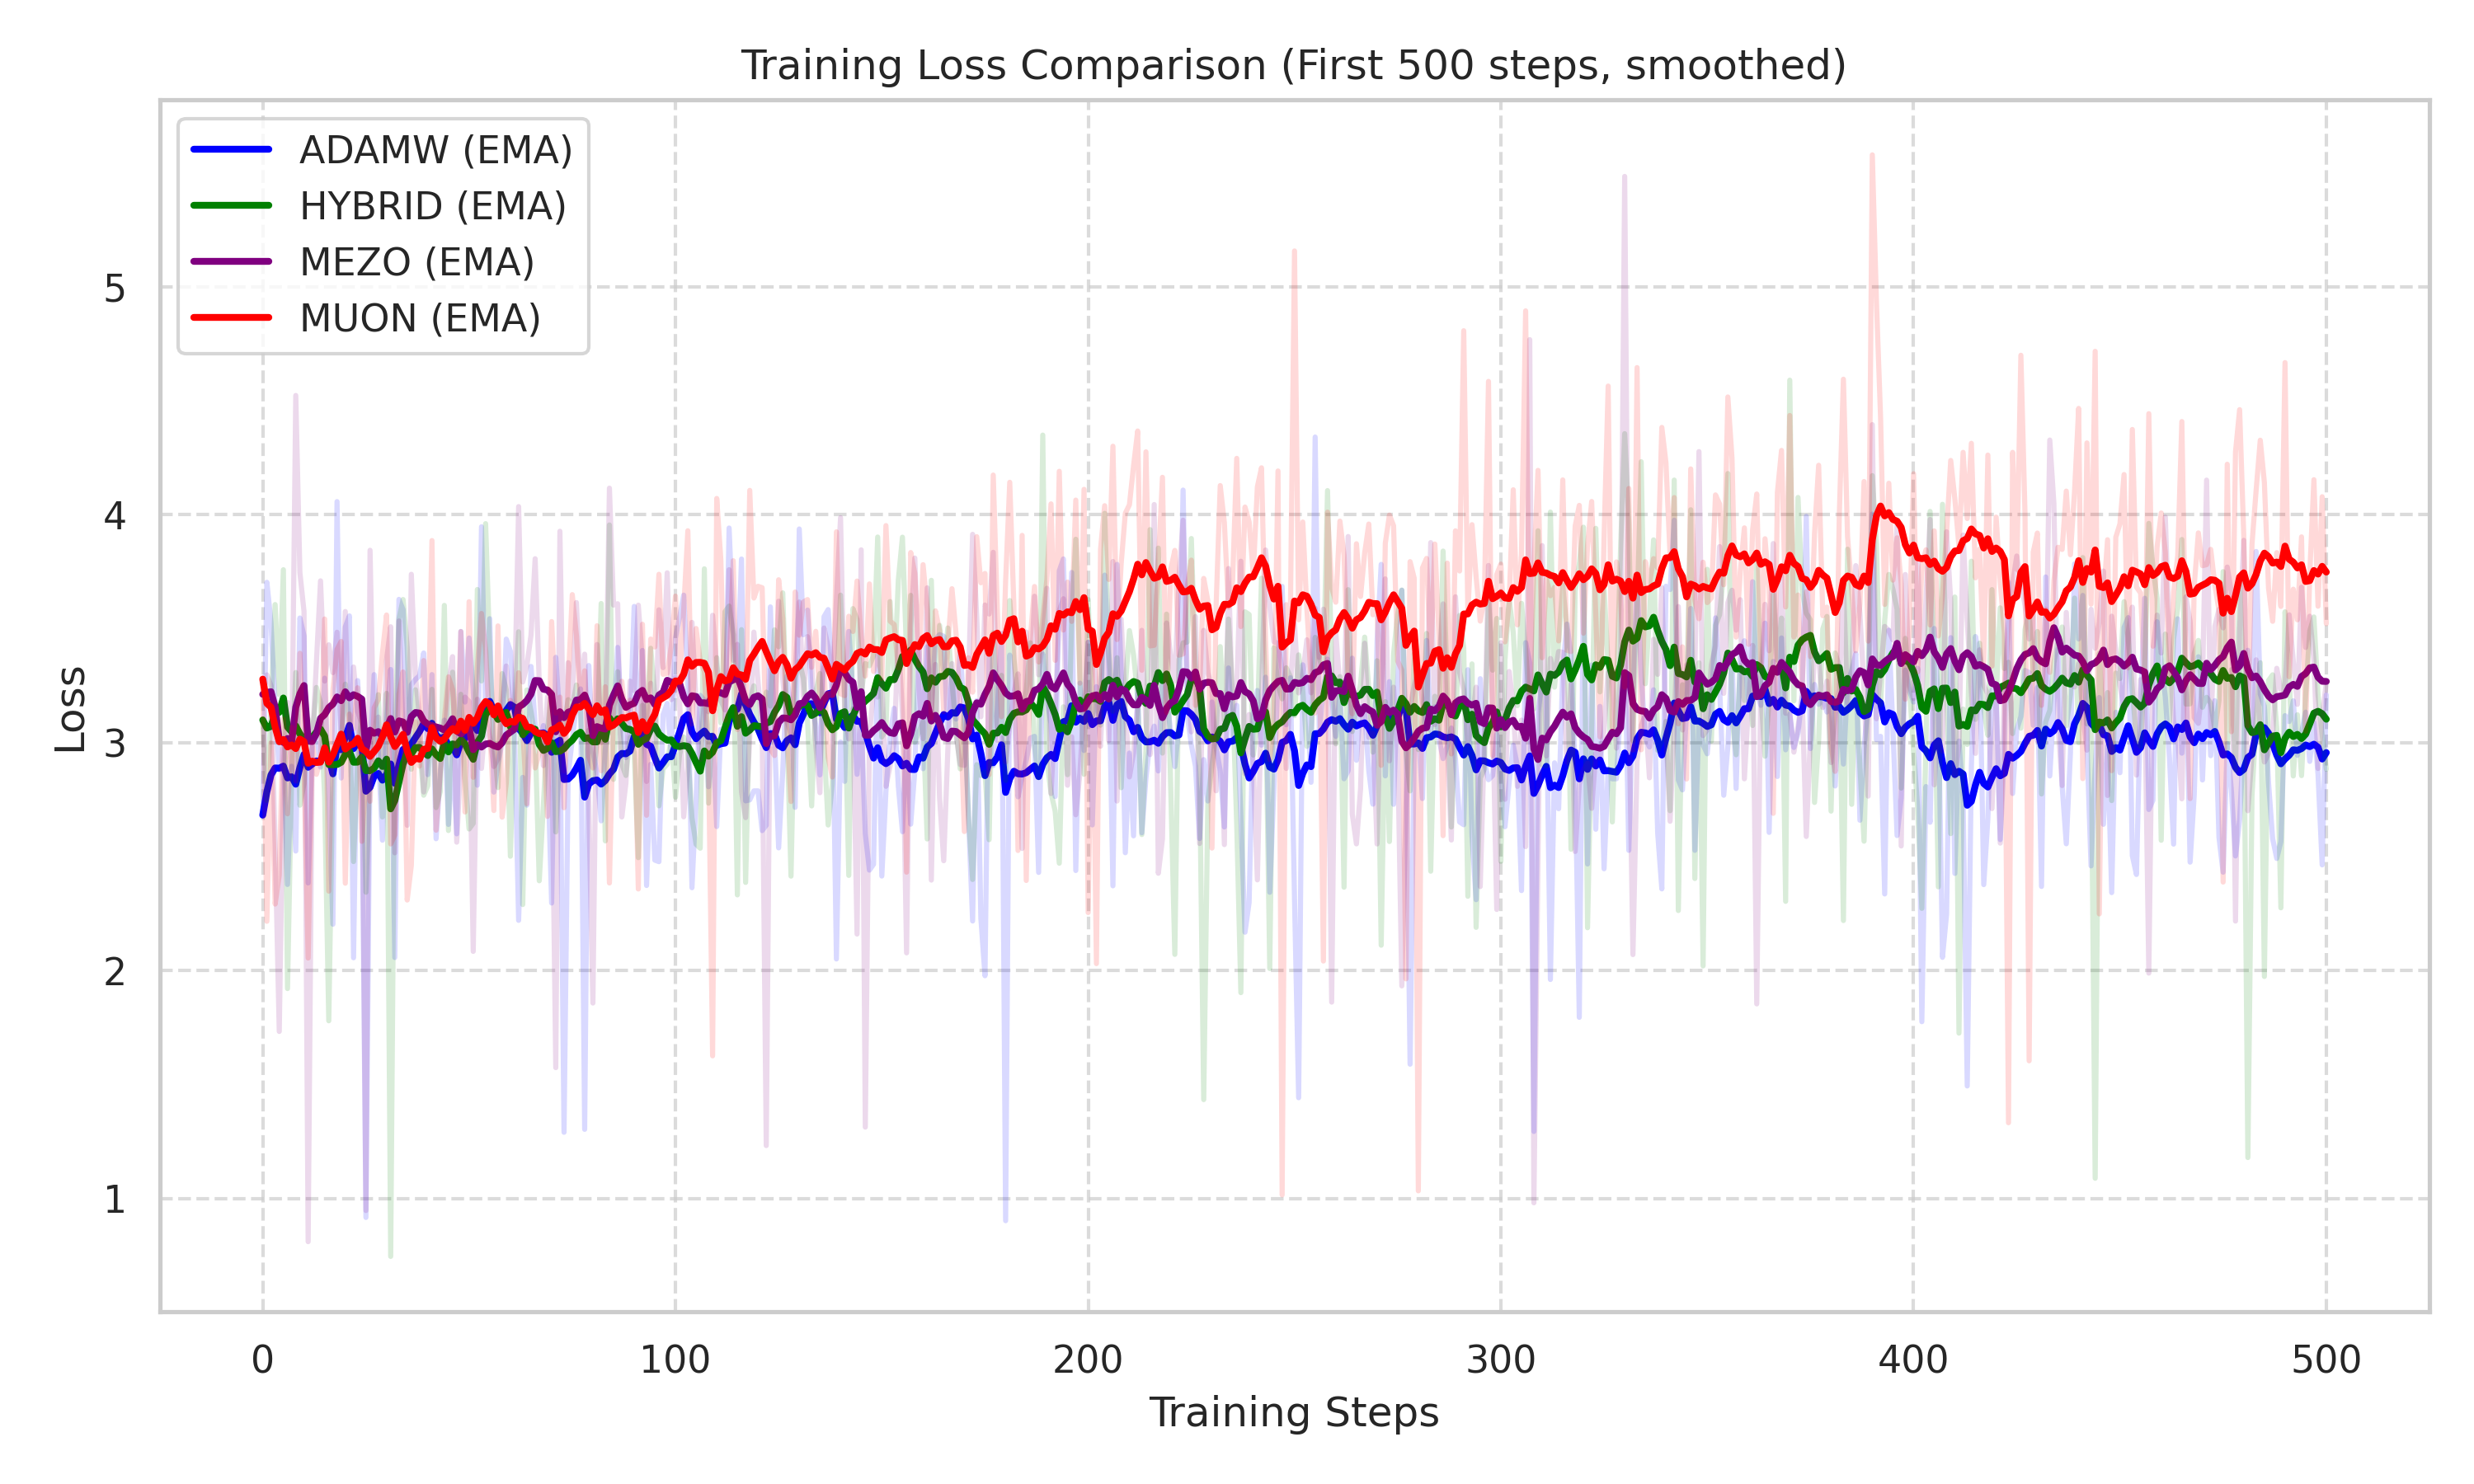
\includegraphics[width=0.8\textwidth]{training_loss.png}
\caption{Smoothed Training Loss comparison. AdamW shows the most stable descent, while Muon and Hybrid exhibit higher initial variance due to weight orthogonalization.}
\label{fig:loss}
\end{figure}

The evaluation results (Table \ref{tab:results}) show a clear trend: standard first-order optimization with AdamW is the most effective for short-term fine-tuning.

\begin{table}[h]
\centering
\begin{tabular}{lccccc}
\toprule
\textbf{Benchmark} & \textbf{Baseline} & \textbf{AdamW} & \textbf{Muon} & \textbf{Hybrid} & \textbf{MeZO} \\
\midrule
ARC-Challenge & \textbf{32.08\%} & 31.65\% & 25.34\% & 23.98\% & 26.71\% \\
ARC-Easy & 58.33\% & \textbf{61.70\%} & 38.97\% & 26.98\% & 25.63\% \\
HellaSwag & \textbf{52.10\%} & 51.82\% & 34.55\% & 25.79\% & 26.01\% \\
PIQA & 69.91\% & \textbf{70.13\%} & 58.97\% & 51.90\% & 49.95\% \\
WinoGrande & 56.11\% & \textbf{57.93\%} & 51.06\% & 50.51\% & 49.41\% \\
\bottomrule
\end{tabular}
\caption{Zero-shot performance (Accuracy / Acc_norm). MeZO results after 15k steps; others after 500 steps.}
\label{tab:results}
\end{table}

Full training logs, containing learning rate, loss, and compute time for every training step across all experiments, are provided in the \texttt{logs/} directory of the repository for full transparency and reproducibility.

AdamW not only preserved knowledge but improved results on ARC-Easy and WinoGrande. Muon, even with a reduced learning rate, caused "catastrophic forgetting," likely because forcing pre-trained weights toward orthogonality disrupts the carefully learned manifolds. MeZO remained near random-chance performance, which is expected given the high dimensionality of the parameter space and the relatively low number of steps (15k) compared to the millions typically required for ZO methods.

\section{Resource Efficiency Analysis}
\begin{itemize}
    \item \textbf{Memory (VRAM):} AdamW, Muon, and Hybrid consumed approximately 6-8 GB of VRAM. MeZO demonstrated a significant advantage, requiring only $\sim$2.5 GB of VRAM, as it does not require storing gradients or intermediate activations for the backward pass.
    \item \textbf{Compute Time:} MeZO is roughly $2 \times$ slower per step than AdamW because it requires two forward passes per update. Muon is slightly slower due to the overhead of Newton-Schulz iterations on the GPU.
\end{itemize}

\section{Conclusion}
While Muon is superior for training from scratch, \textbf{AdamW remains the preferred choice for fine-tuning} due to its ability to maintain pre-trained representations. The Hybrid approach requires extremely careful per-group LR tuning to avoid divergence. MeZO is a powerful tool for OOM scenarios but requires a significantly higher step budget to achieve competitive accuracy.

\end{document}